\documentclass[12pt]{article}
\usepackage[a4paper, left=3.17cm, right=3.17cm, top=2.54cm, bottom=2.54cm]{geometry}
\usepackage[fontset=mac]{ctex}
\usepackage[T1]{fontenc}
\usepackage{mathptmx}
\usepackage{amsfonts}
\usepackage{amsmath,amssymb,amsthm}
\usepackage{enumerate}
\usepackage{graphics}
\usepackage{chemformula}
\usepackage{cite}
\usepackage[colorlinks, linkcolor=black, anchorcolor=black, citecolor=black]{hyperref}
\usepackage{indentfirst}

\usepackage{graphicx}
\setlength{\parskip}{0.5em}
\title{《高性能计算引论》第二次作业}
\author{\textup{罗文水}}
\begin{document}
	
	\begin{titlepage}
		\newcommand{\HRule}{\rule{\linewidth}{0.5mm}}
		\begin{center}
			
\includegraphics[width=8cm]{../HPC_P1/title}			
		\end{center}
		
		\center 
		\quad\\[1.5cm]
		\textsl{\Large \textbf{Nanjing University of Science and Technology} }\\[0.5cm] 
		\textsl{\large School of Computer Science and Engineering}\\[0.5cm] 
		\makeatletter
		\HRule \\[0.4cm]
		{ \huge \bfseries \@title}\\[0.25cm] 
		\HRule \\[1.5cm]
	\begin{minipage}{0.42\textwidth}
		\begin{flushleft}
			
			\Large{\emph{姓名:罗文水}}
			\\
			\Large{\emph{学号:918106840738}}
			\\
			\Large{\emph{班级:计科一班}}
			\\
			\Large{\emph{课程:高性能计算引论}}
			\\
			\Large{\emph{授课教师:李翔宇}}
			\\
		\end{flushleft}
	\end{minipage}
		\vspace{7em} 
		
		{\large \today}\\[2cm] 
		\vfill 
	\end{titlepage}
	
	\newpage
\section{问题一}
	\begin{figure}[h]
		\centering
		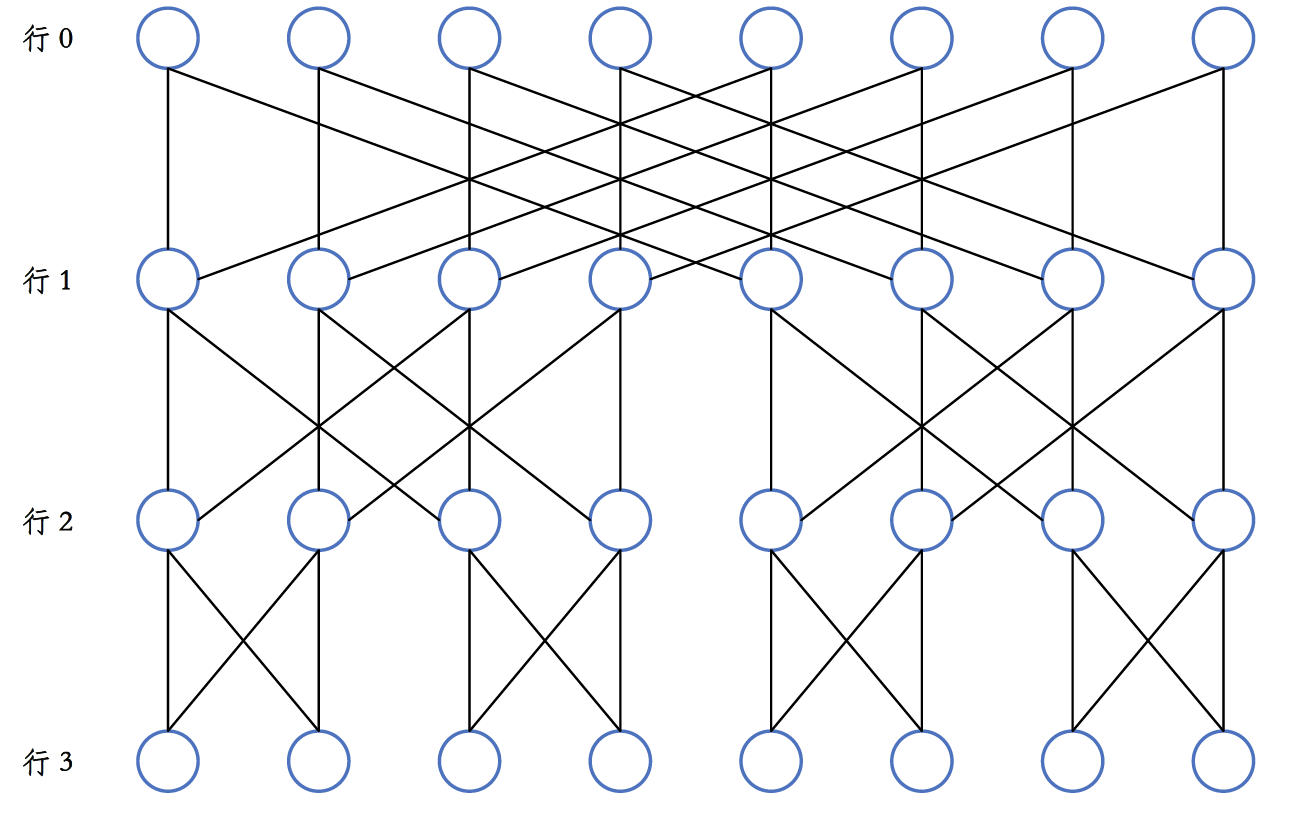
\includegraphics[width=1.0\textwidth]{network.png}
		\caption{三层蝶形网络结构图}
	\end{figure}
	该网络的各项参数如下所示:
	\begin{enumerate}
		\item \textbf{网络直径}:大小为$(k+1)\cdot 2^k$的网络的直径为$2k$。
		
		\textbf{证明:}假设第$i$行从左至右分别按照二进制位进行编号,
		编号记为:$${a^{(i)}_{k-1}a^{(i)}_{k-2}a^{(i)}_{k-3}\dotsb a_0^{(i)}}$$ 
		则蝶形网络第$s$行与第$s+1$行之间的互联逻辑为如下蝶形函数(即将第s层的输入元$m$第s位取反,变为$m'$,
		并建立$m$到$m'$之间的连接。
		\begin{equation}
			\epsilon_{s}(x^{(s)})=x^{(s)}_{k-1}x^{(s)}_{k-2}\dotsb \overline{x^{(s)}_{k-1-s}} \dotsb x^{(s)}_{0}
		\end{equation}
		或者,在两层之间,编号相同的同样建立连接。连接函数如下:
		\begin{equation}
			\epsilon_{s}(x^{(s)})=x^{(s)}_{k-1}x^{(s)}_{k-2}\dotsb x^{(s)}_{k-1-s} \dotsb x^{(s)}_{0}=x^{(s)}
		\end{equation}
		根据上述公式,从第0行中选择一个编号为$m^{(0)}$的节点,从第$k+1$行中选择一个编号为$\overline{m}^{(k)} $的编号,该编号的二进制位为$m$的每一位取反,
		并选择一个编号与$m^{(0)}$相同的节点$m^{(k)}$,则$m^{(0)}$与$\overline{m}^{(k)} $之间的距离一定为k,即通过k次二进制位取反可以得到,其次,
		从$m^{(0)}$到$m^{(k)}$,二进制位不变,也存在一条从第0行到第$k$行的长度为$k$的路径,当取$m^{(0)}=000\dotsb00$时,从$m^{(k)}$节点到$\overline{m}^{(k)} $
		之间的距离为$2\cdot k$。且由于网络中的节点都是通过变换二进制位进行连接,从而任意两个节点之间的距离不能超过$2\cdot k$ ,故该网络的直径是$2\cdot k$。
		\item \textbf{等分宽度}:该网络的等分宽度为$2^{k}$。
		
		\textbf{证明:}按照第一问的分析方法,第0层到第1层之间的互联函数
		实现的逻辑功能是$\epsilon_0(x^{(0)})$,即将最高位取反。如果考虑将网络划分为左右两部分,则在网络左边以及右边组内编号的二进制位首位相同。
		由于互联函数中只有$\epsilon_0(x^{(0)})$可以改变高位,其他函数$\epsilon_s(x^{(s)}) \quad \forall \;s \neq 0$都是指在组内
		进行连接,故对于计算两组之间的link数量,只需要计算互联函数$\epsilon_0(x^{(0)})$连接的边数量,由于该函数是作用在第0层上的,而
		第0层一共有$2^{k}$个结点,所以可以通过删除$2^{k}$条边使得网络等分为两个相同节点数的网络。而分割该网络为两个相同大小的子网络,必须至少分割$2^{k}$条link,
		故一个层数为$k$的蝶形网络等分宽度为$2^{k}$。
		\item \textbf{边连通度}:一个层数为$k$的蝶形网络的边连通度为2。
		
		\textbf{证明:}从蝶形网络的构造上来看,只有第一层和最后一层的节点度为2,其他节点的节点度都为4,即对第0层的节点$x$而言,$x$连接第二层的link代表两种选择,分别是高位不变与高位取反。
		将两个link删除即可将$x$从网络中分离出来。而至少要删除2条link才能使网络不连通。从而该网络的节点度为2。
	\end{enumerate}
\newpage
\section{问题二}
		(1)运行Hello World程序三次得到的结果分别如下所示。
		\begin{figure}[htbp]
			\centering
			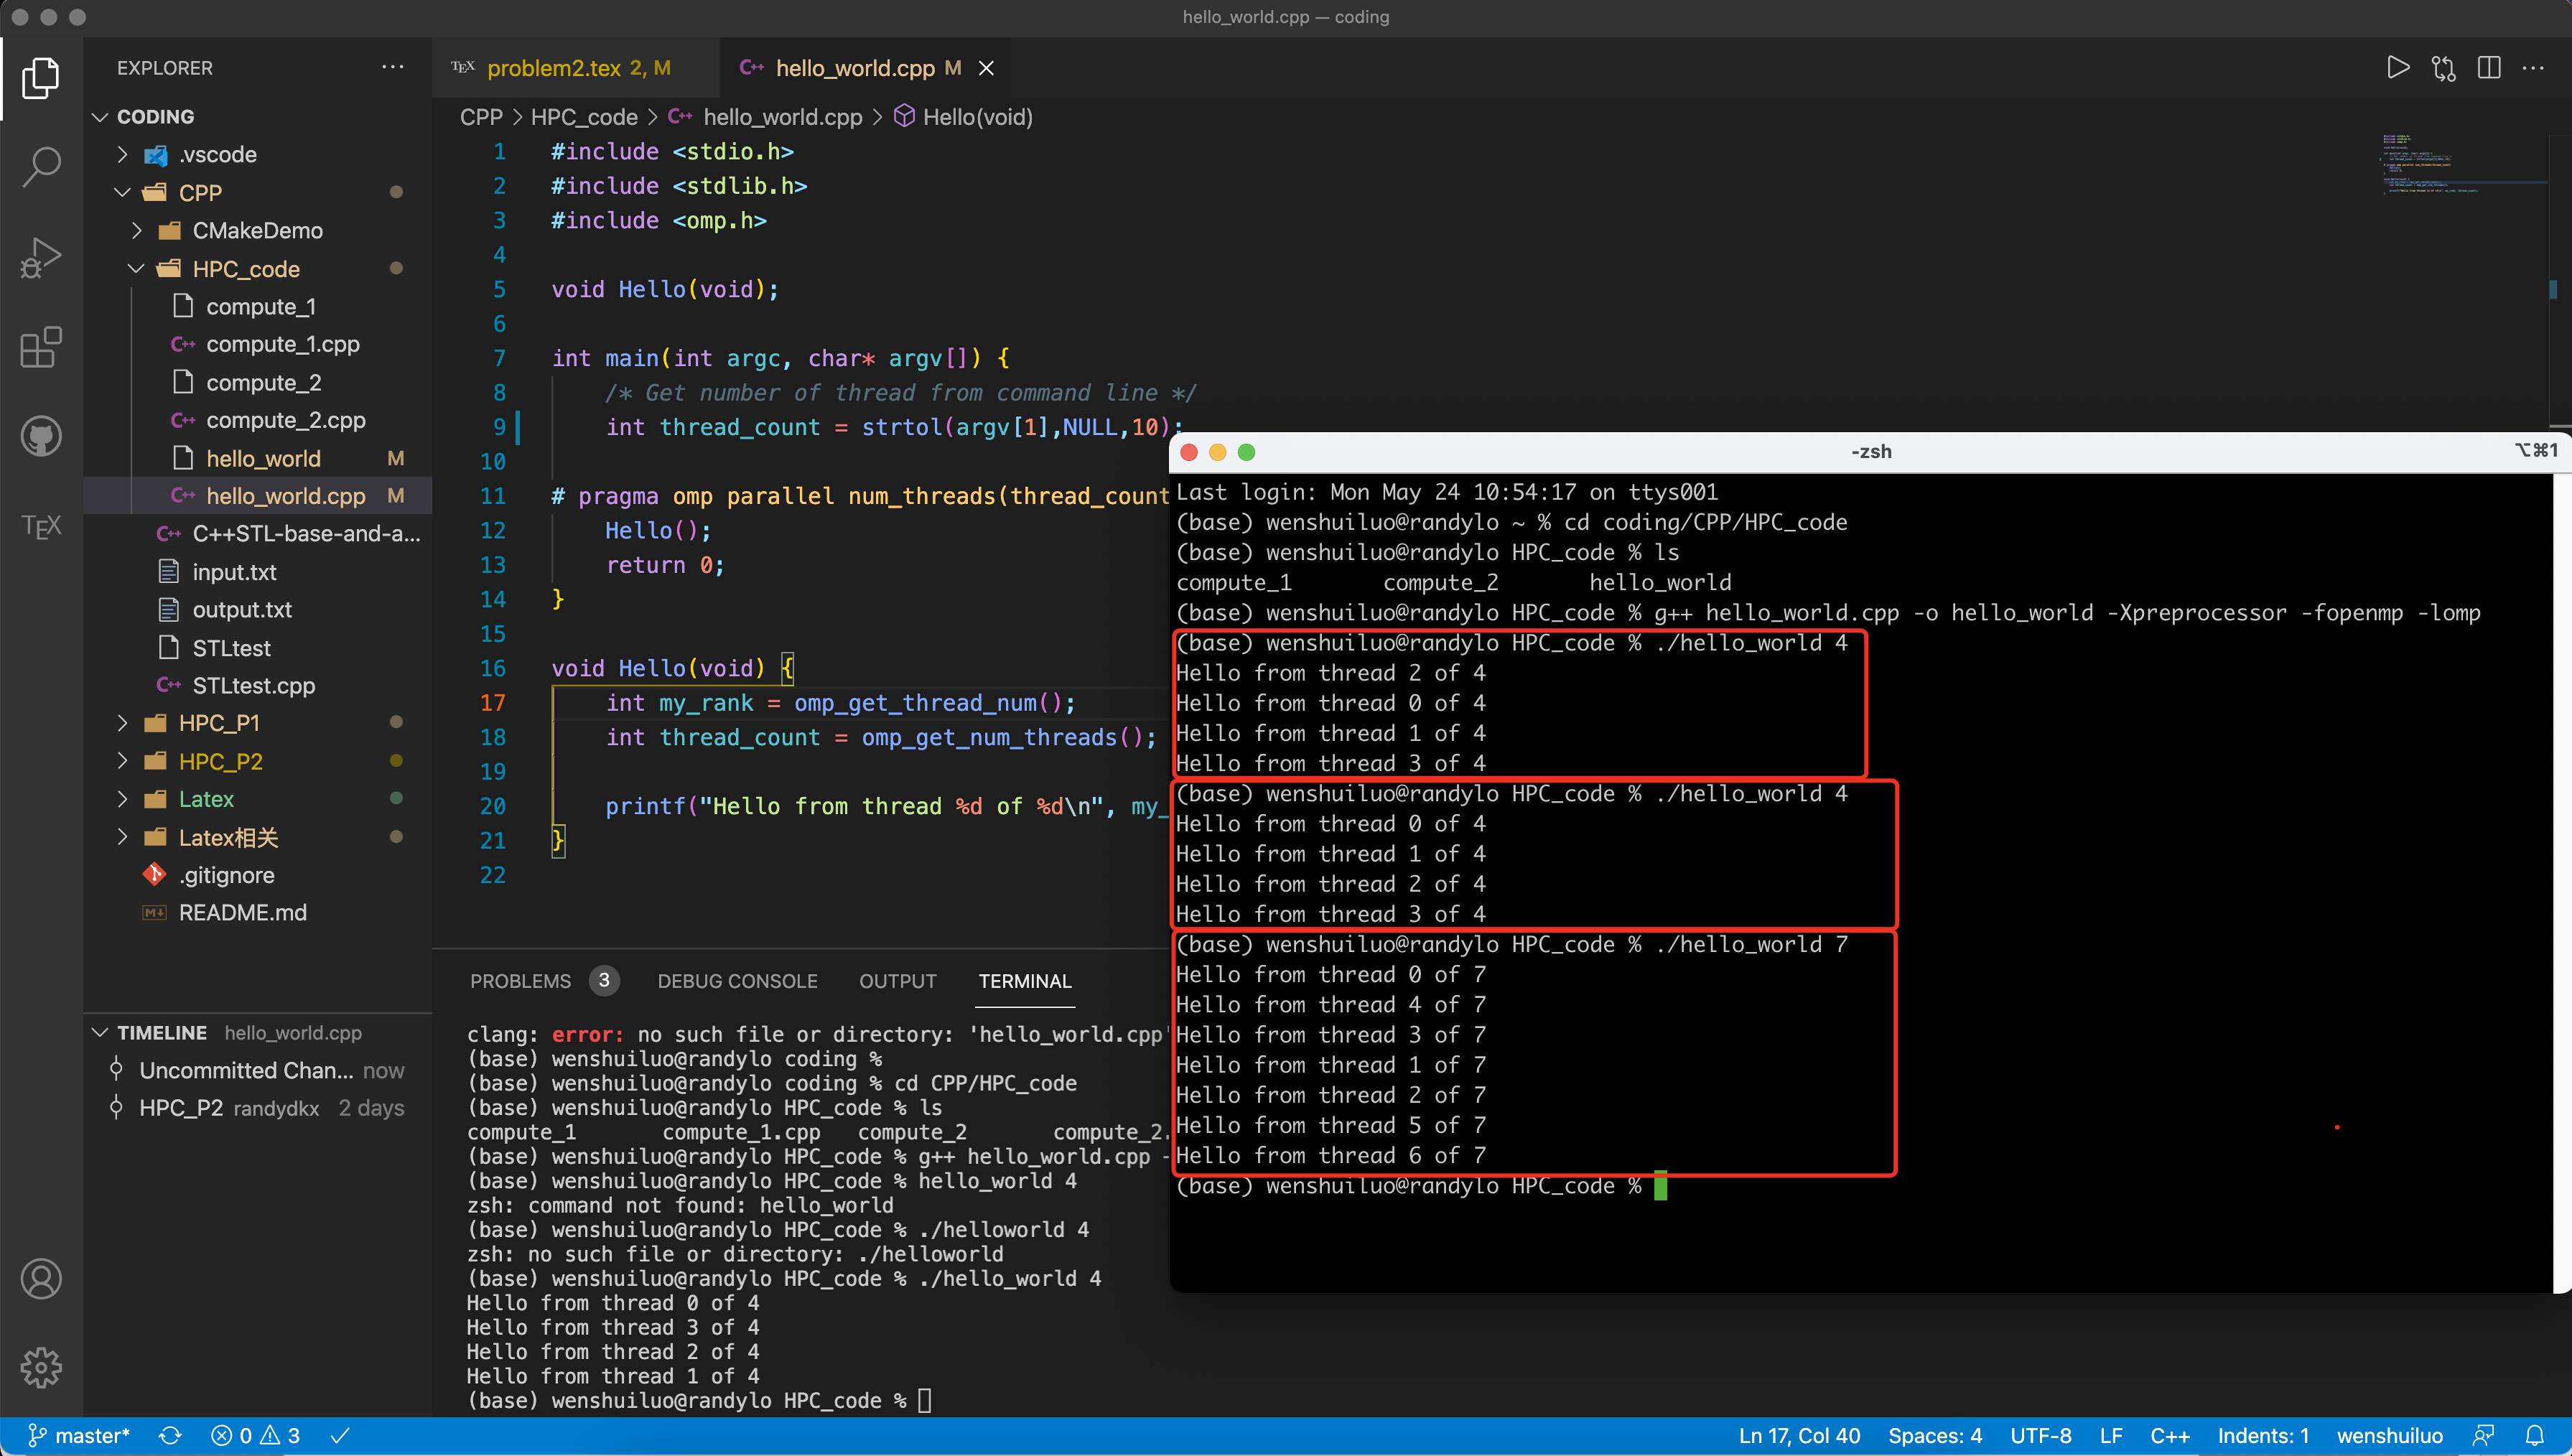
\includegraphics[width=0.9\textwidth]{hello_world三次运行.png}
			\caption{问题一三次运行截图1}
			\label{fig:pro2_1_1}
		\end{figure}
		\begin{figure}[htbp]
			\centering
			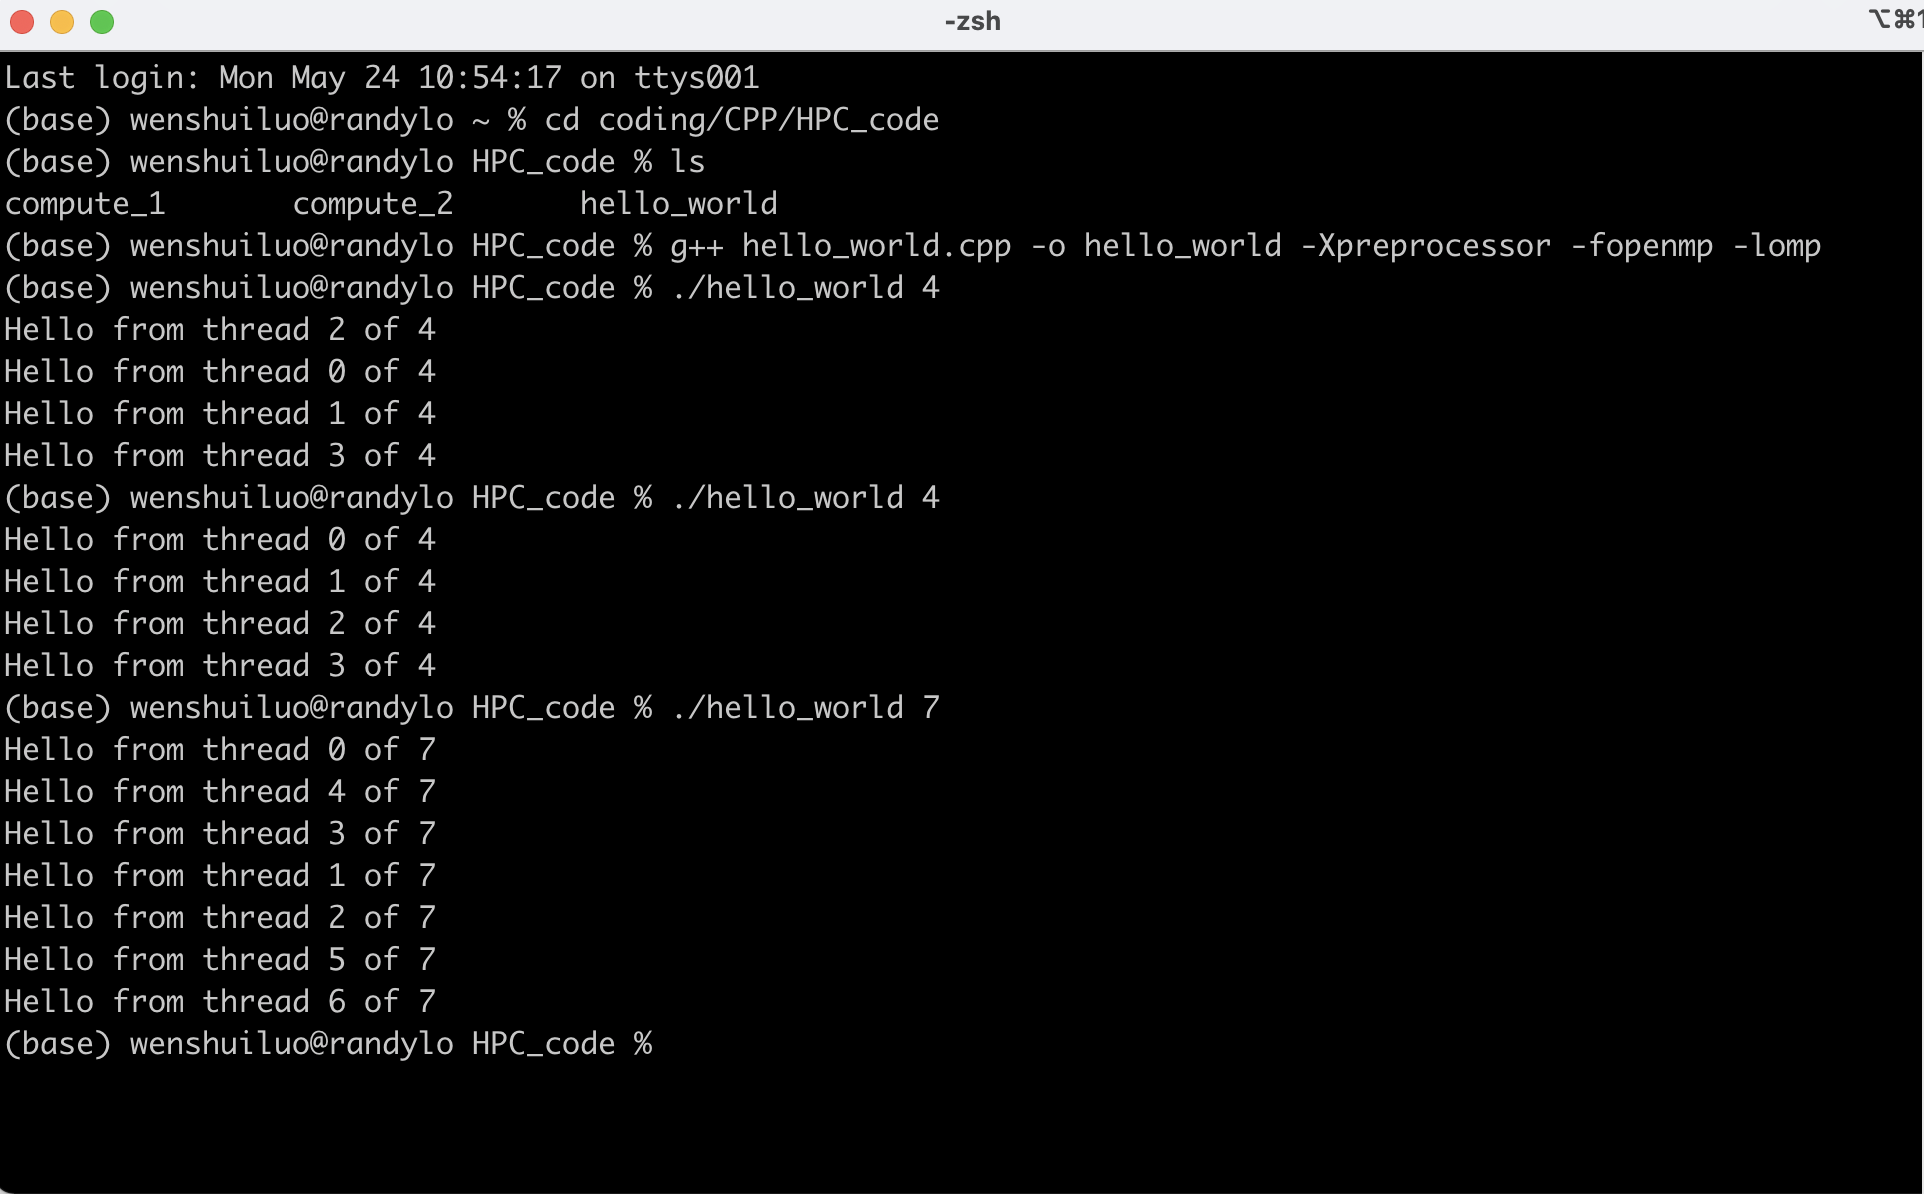
\includegraphics[width=0.9\textwidth]{pro1.png}
			\caption{问题一三次运行截图2}
			\label{fig:pro2_1_2}
		\end{figure}

		从图1和图2中可知三次运行hello world程序分别启动了4、4、7个线程,对于每次执行,每个线程都执行打印hello\_world程序。
		由于线程之间的顺序推进不一致,在第一次执行和第二次执行中,程序的打印结果不同。每个线程只执行打印hello代码块一次,故对于$k$个线程会有$k$相应的排列输出。		

		(2) 两段程序的执行结果分别如下图所示
		\begin{figure}[htbp]
			\centering
			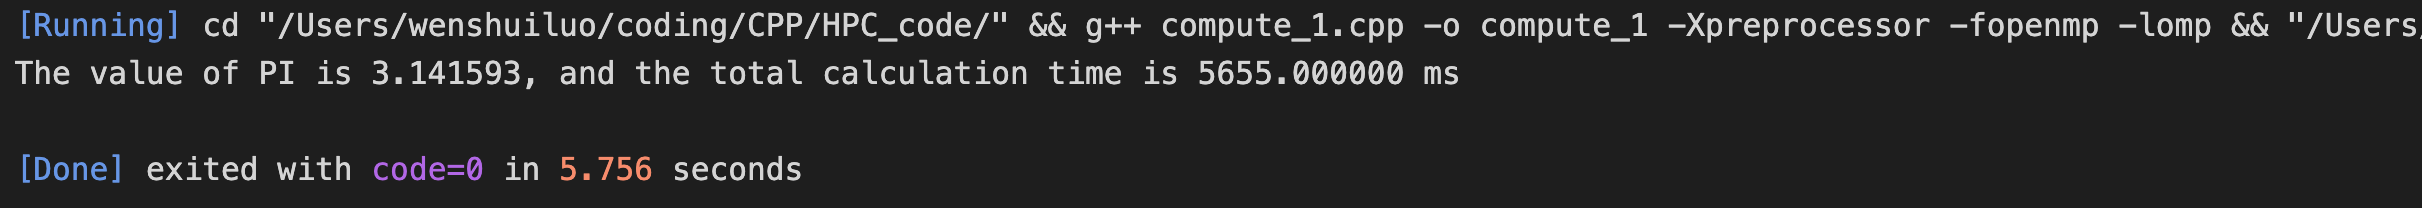
\includegraphics[width=1.0\textwidth]{result4.png}
			\caption{(2)未采用并行方法执行的结果}
		\end{figure}
		
		\begin{figure}[htbp]
			\centering
			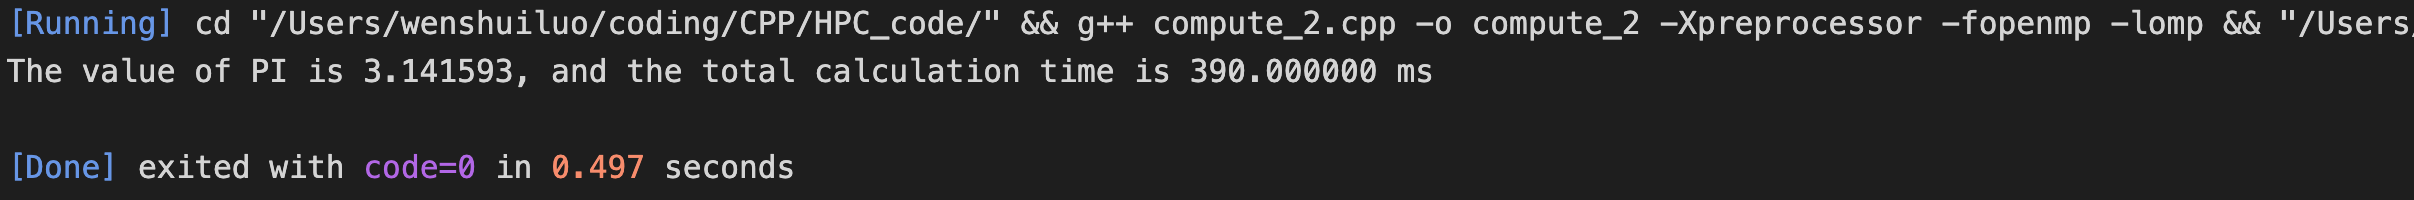
\includegraphics[width=1.0\textwidth]{result5.png}
			\caption{(2)采用并行方法执行的结果}
		\end{figure}

		从中可见未执行并行计算的程序计算时间长达$5655ms$,并行计算的程序执行时间只有$390ms$,性能上是未并行程序的十几倍。极大地缩短了计算时间,通过计算得知,执行时间上多线程执行时间与单线程执行时间比例$\frac{390}{5655}\approx \frac{1}{14.5}$,故大约启用了14个线程执行执行$\pi$值的计算,根据本机配置(本机为8核心16线程多核系统),大约启用14个内核线程进行并行计算。

		程序的完整执行如图6与图7所示。
		\begin{figure}[p]
			\centering
			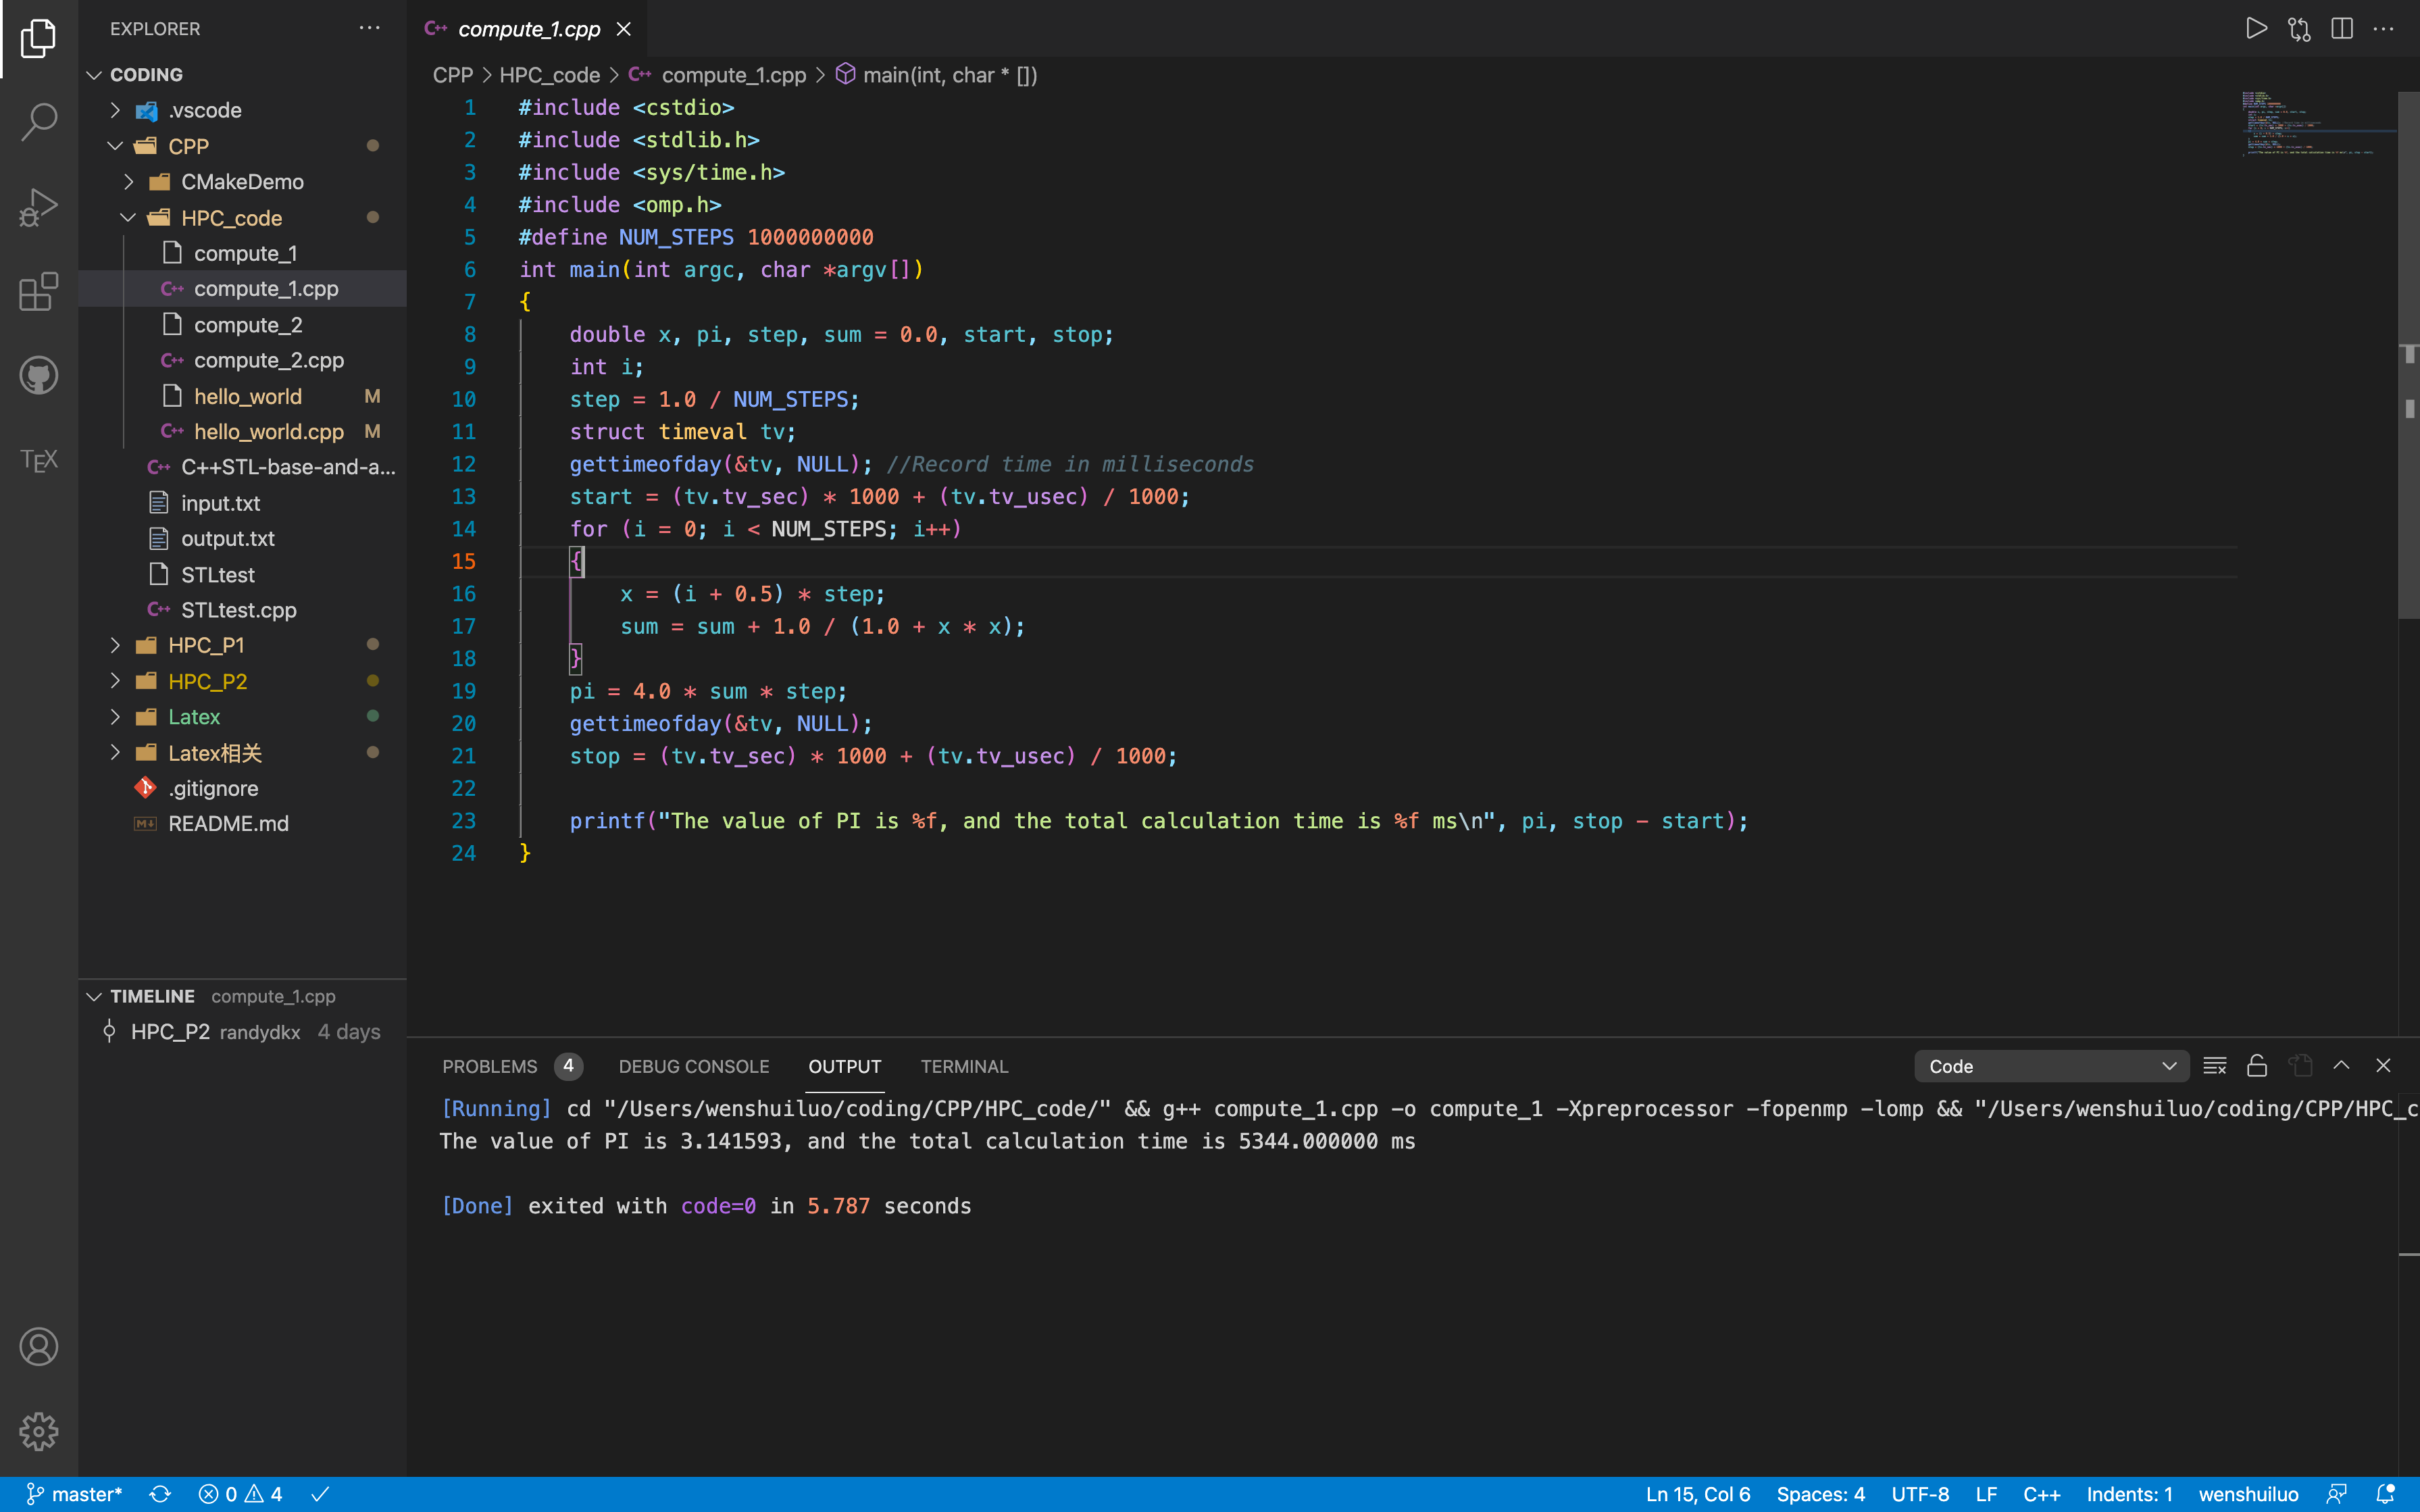
\includegraphics[width=1.0\textwidth]{1_1.png}
			\caption{单线程串行:完整执行}
		\end{figure}

		\begin{figure}
			\centering
			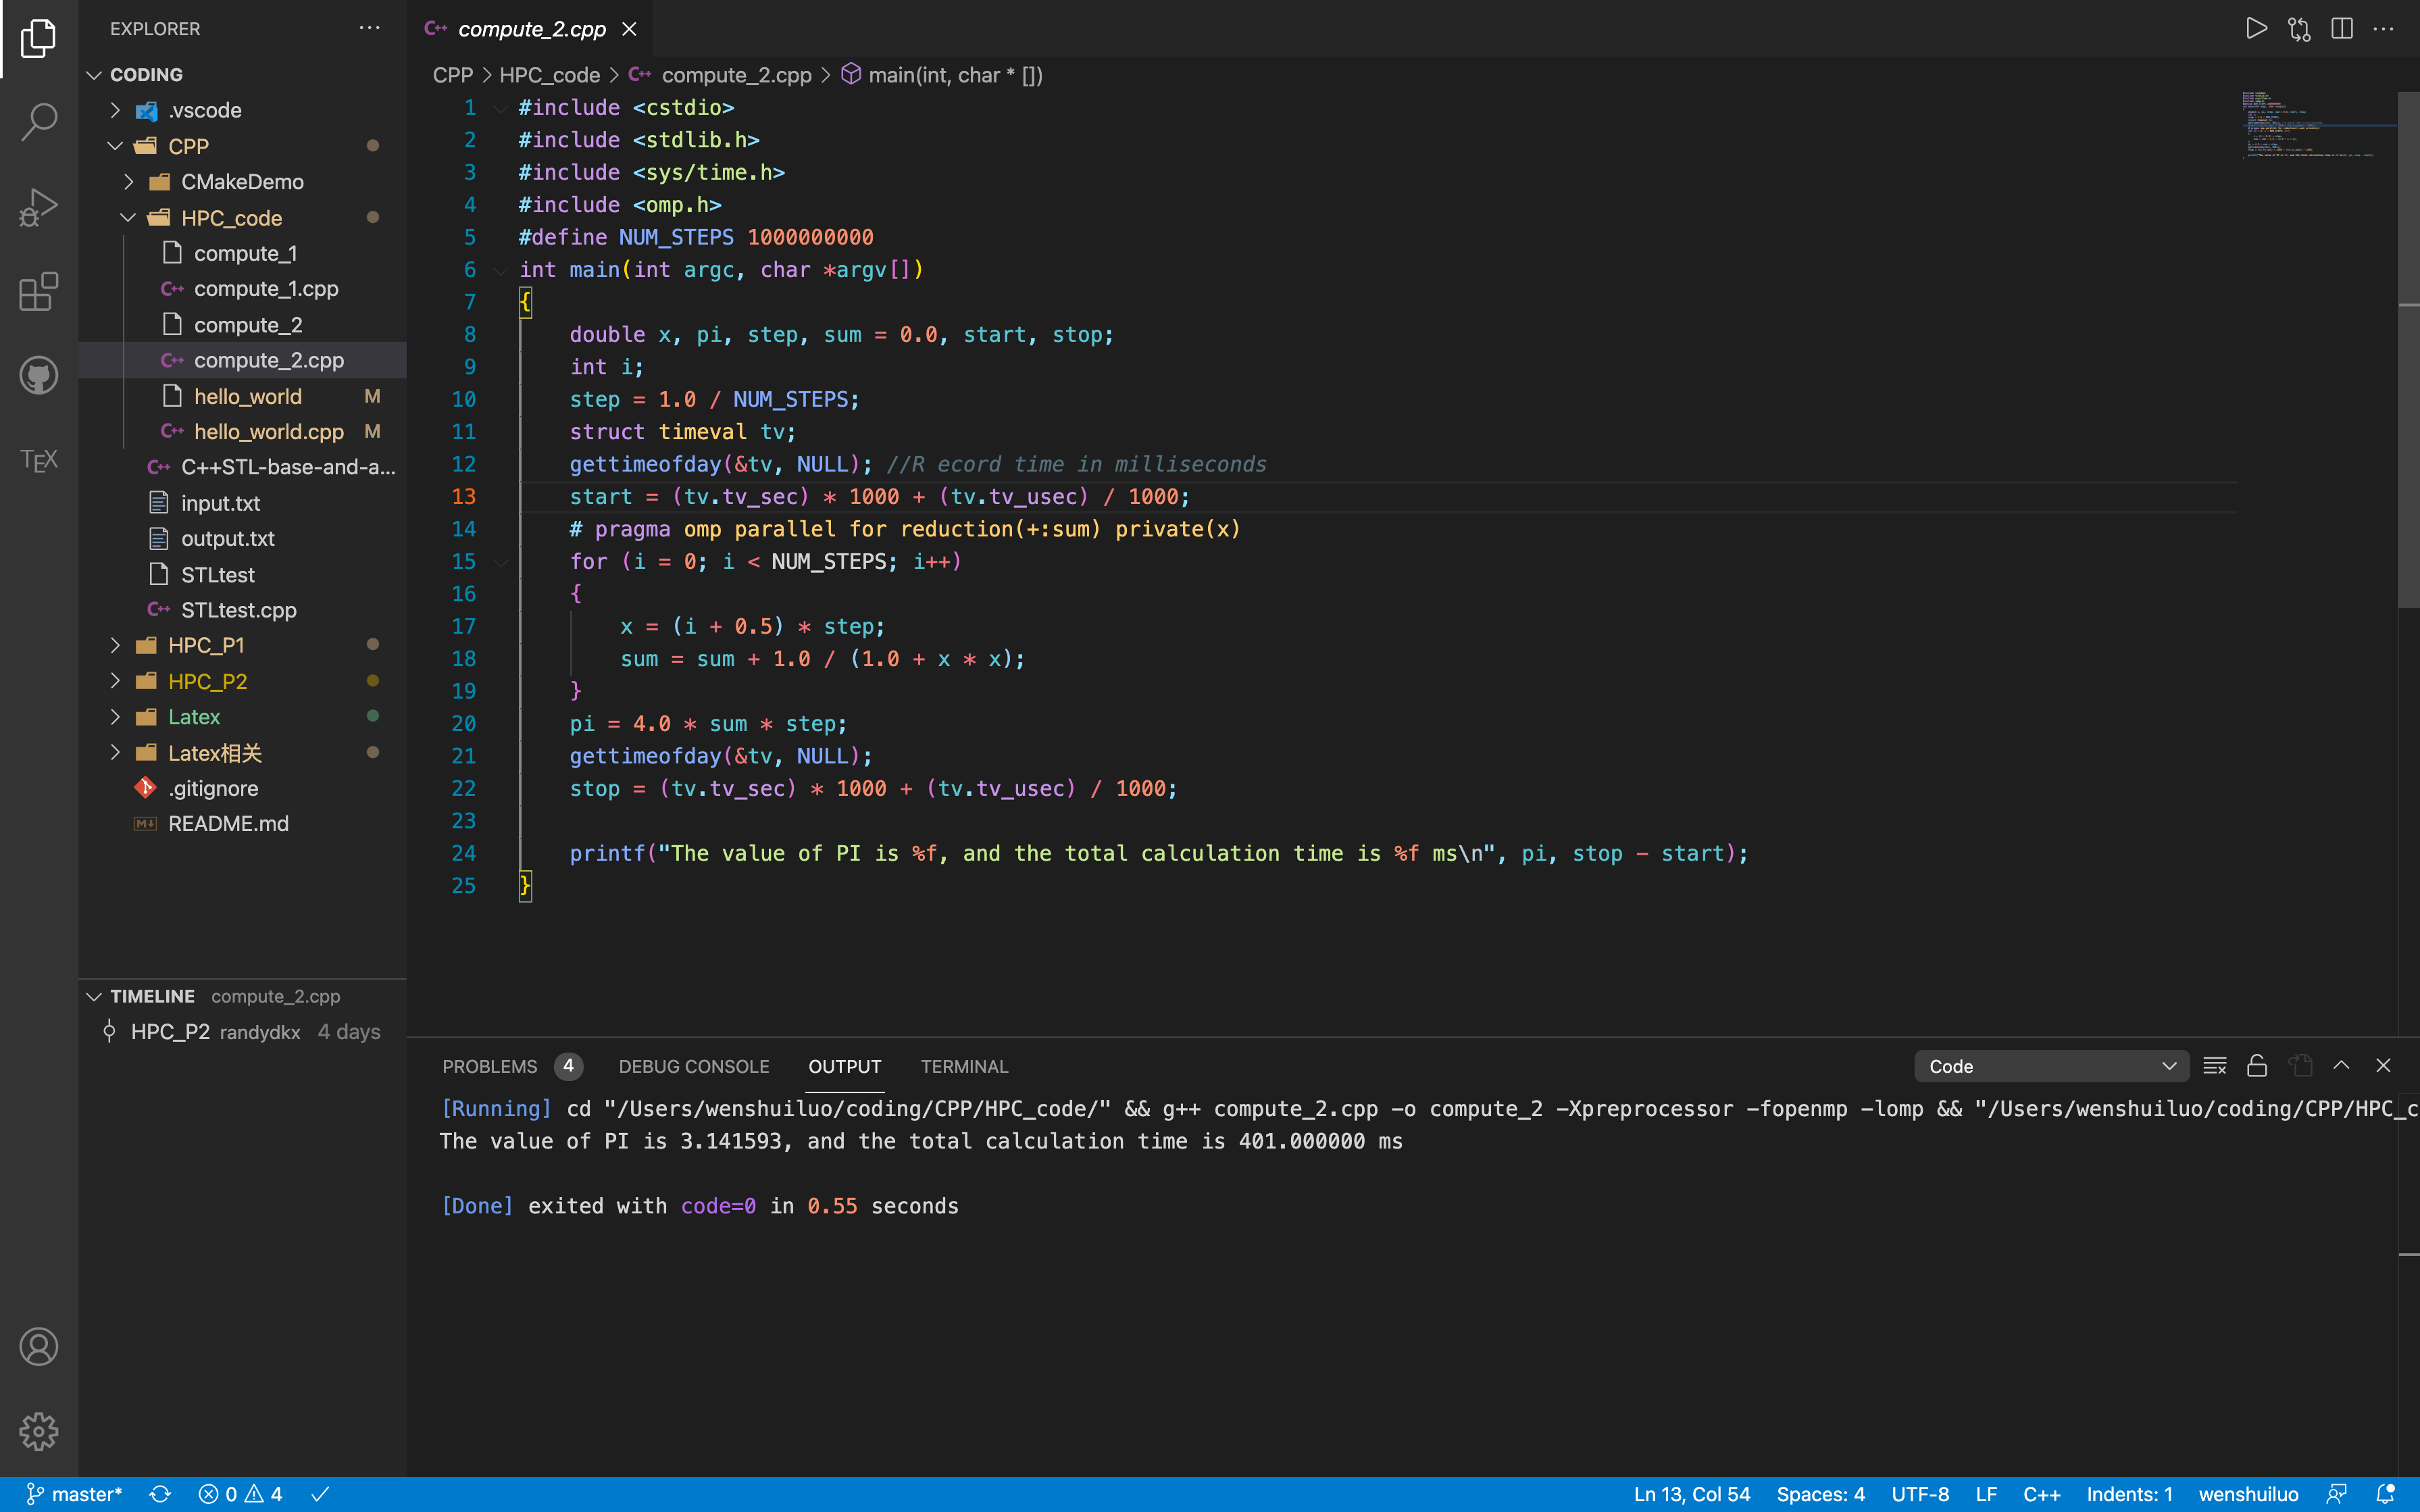
\includegraphics[width=1.0\textwidth]{1_2.png}
			\caption{多线程并行:完整执行}
		\end{figure}
	
\end{document}
